\documentclass[review]{elsarticle}

\usepackage{lineno}
\usepackage[hidelinks]{hyperref}
\modulolinenumbers[5]

\usepackage{amsmath,amsthm,amssymb,mathrsfs}

\journal{Journal of Combinatorial Theory, Series A}

%%%%%%%%%%%%%%%%%%%%%%%
%% Elsevier bibliography styles
%%%%%%%%%%%%%%%%%%%%%%%
%% To change the style, put a % in front of the second line of the current style and
%% remove the % from the second line of the style you would like to use.
%%%%%%%%%%%%%%%%%%%%%%%

%% Numbered
%\bibliographystyle{model1-num-names}

%% Numbered without titles
%\bibliographystyle{model1a-num-names}

%% Harvard
%\bibliographystyle{model2-names.bst}\biboptions{authoryear}

%% Vancouver numbered
%\usepackage{numcompress}\bibliographystyle{model3-num-names}

%% Vancouver name/year
%\usepackage{numcompress}\bibliographystyle{model4-names}\biboptions{authoryear}

%% APA style
%\bibliographystyle{model5-names}\biboptions{authoryear}

%% AMA style
%\usepackage{numcompress}\bibliographystyle{model6-num-names}

%% `Elsevier LaTeX' style
\bibliographystyle{elsarticle-num}
%%%%%%%%%%%%%%%%%%%%%%%

%% Ticketing System
\usepackage{etoolbox}
\usepackage{xparse}
\NewDocumentCommand{\openTickets}{ > {\SplitList {,} } m }{\ProcessList{#1}{\BoolInit}}
\newcommand{\BoolInit}[1]{\providetoggle{#1}\toggletrue{#1}}
\newcommand{\todo}[2]{%
  \providetoggle{#1}%
    \iftoggle{#1}{%
    {\color{red}#2}%
    }{#2}%
}

\usepackage{tikz}
\usetikzlibrary{arrows,positioning,patterns,decorations.pathreplacing}


%% Ticket list
\openTickets{Manuel:convHull,Manuel:wlog,Manuel:invertability:assumption,Mark:log:bounds,Mark:proof:cor15,Manuel:proof:rewritten,Manuel:generic}


\providecommand{\norm}[1]{\left\|#1\right\|}
\providecommand{\abs}[1]{\left|#1\right|}
\providecommand{\span}{\text{span}}
\providecommand{\conv}{\text{conv}}
\providecommand{\epi}{\text{epi}}
\providecommand{\rk}[1]{\text{rank}\left(#1\right)}

\newcommand*{\Resize}[1]{\resizebox{\columnwidth}{!}{$#1$}}

\newcounter{thmcount}
\renewcommand{\thethmcount}{\arabic{thmcount}}
\renewcommand{\theequation}{\arabic{section}.\arabic{equation}}
\renewcommand{\thefigure}{\arabic{section}.\arabic{figure}}


\newtheorem{thm}[thmcount]{Theorem}
\newtheorem{cor}[thmcount]{Corollary}
\newtheorem{prop}[thmcount]{Proposition}

\theoremstyle{remark}
\newtheorem{rem}[thmcount]{Remark}

\theoremstyle{definition}
\newtheorem{defi}[thmcount]{Definition}
\newtheorem{alg}[thmcount]{Algorithm}

\DeclareFontFamily{U}{mathx}{\hyphenchar\font45}
\DeclareFontShape{U}{mathx}{m}{n}{
      <5> <6> <7> <8> <9> <10> gen * mathx
      <10.95> mathx10 <12> <14.4> <17.28> <20.74> <24.88> mathx12
      }{}
\DeclareSymbolFont{mathx}{U}{mathx}{m}{n}
\DeclareFontSubstitution{U}{mathx}{m}{n}
\DeclareMathSymbol{\temp}{\mathbin}{mathx}{'341}
\newcommand{\bigominus}{\raisebox{10pt}{$\temp$}}

% \newcommand{\todo}[1]{\textcolor{blue}{#1}}
\newcommand{\highlight}[1]{\textcolor{red}{#1}}




\begin{document}

\begin{frontmatter}

\title{Operations on Parametrised Polytopes\tnoteref{mytitlenote}}
\tnotetext[mytitlenote]{Fully documented templates are available in the elsarticle package on \href{http://www.ctan.org/tex-archive/macros/latex/contrib/elsarticle}{CTAN}.}

%% or include affiliations in footnotes:
\author{Rainer M. Schaich}
\ead{rainer.schaich@eng.ox.ac.uk}

\author{Mark Cannon\corref{correspondingauthor}}
\ead{mark.cannon@eng.ox.ac.uk}

\cortext[correspondingauthor]{Corresponding author}


\address{Department of Engineering Science, University of Oxford, Parks Road, OX1 3PJ, Oxford}


\begin{abstract}
The abstract goes here.
\end{abstract}

\begin{keyword}
keyword one \sep keyword two
\end{keyword}

\end{frontmatter}

\linenumbers

\section{Introduction}

%
Notation:~$\mathscr P(X)$ denotes the power set of $X$.
%
\section{Preliminaries}

Throughout the paper we deal with set-valued maps, i.e. functions that map an element of a metric space~$Y$ to a subset of a metric space~$Z$: $f:Y\mapsto\mathscr P(Z), Y\ni y\rightarrow f(y)\subset Z$. 
%
A detailed presentation on properties of set-valued maps is beyond the scope of this paper and we refer to~\cite{Aubin:2009}, here we only assume that the set-valued map is continuous in the sense that its \emph{graph}
%
\begin{equation}
  \mathscr G(f) = \{(y,z)\in Y\times Z: z\in f(y)\}
\end{equation}
%
has a continuous boundary, for every bounded point $(y,z)\in\partial\mathscr G(f)$ the boundary $\partial\mathscr G(f)$ is locally given by the graph of a continuous function.
%
We only consider set-valued maps with convex images, i.e. such maps for which $z_1,z_2\in f(y)\Rightarrow \lambda z_1+(1-\lambda)z_2\in f(y)$ for all $\lambda\in[0,1]$ holds for all $y\in Y$.

An important subset of such set-valued maps are such that their realisations are polytopic, $f(y)$ is a polytope for all $y\in Y$, in particular we study maps which depend on the \emph{parameter} in a piecewise affine way.
%
The graph of such maps is given by a union of polytopes, they have been studied in~\cite{Finzel:2000}.
%
We will make statements about \emph{generic} such maps, that is properties which are structurally stable in the sense that if~$f(y)$ has a particular property than there exists an open neighbourhood $U\ni y$ such that $f(\tilde y)$ has the same property for all $\tilde y\in U$, furthermore the set of points for which the property does not hold is of measure zero.
%
In the course of this paper it will be self evident what the set of points is, where the property of interest fails, in particular a lower dimensional polyhedron and we therefore omit a measure theoretic treatment of our assumption.

The particular property we require is \emph{simplicity}, for each $y\in Y$ the set $f(y)$ is a polytope and each of its vertices~$v(y)$ is supported by a minimal number of hyperplanes, i.e. there exists linear system defining the set~$f(y) = \{z:A(y)z\leq b(y)\}$ and each vertex $v(y)$ is defined by $dim(Z)$ hyperplanes $A_{\mathcal I}(y)v(y)=b_{\mathcal I}(y)$ and $A_{\bar{\mathcal I}}(y)v(y)<b_{\bar{\mathcal I}}(y)$.
%
It is easy to see, that if $A(\cdot)$ and $b(\cdot)$ are continuous in $y$, then $\mathcal I$ locally defines a vertex, i.e. the combinatorial structure of a simple polytope is structurally stable and therefore being simple is a generic property of a polytope.


The induced graph~$G(P)$ of a polytope~$P$ is the graph for which the vertices and edges coincide with the vertices and edges of the polytope itself~\cite{Bondy:2008}.
%
In this paper we only use one property of induced graphs, namely the \emph{Perles' Conjecture}~\cite{Kalai:1988}:
\emph{For a simple polytope~$P$ the graph~$G(P)$ determines the combinatorial structure of~$P$.}

\section{Parametric Convexity}

In this section we define the property of \emph{parametric convexity} in the context of set-valued maps. 
%
This property is then used to demonstrate the convexity of a generalised Pontryagin difference (see e.g.~\cite{blanchini:2007}). 
%
In this section we refer to sets $Y\subseteq\mathbb R^d$ and $Z\subseteq\mathbb R^n$.
%
\begin{defi}[Parametric Convexity]\label{def:parametric:convexity}
Let $\mathcal W:Y\rightarrow \mathscr P(Z)$, where $Y\ni p\mapsto \mathcal W(p) \subset Z$, be a continuous set-valued map. The map $\mathcal W$ is called \emph{parametrically convex} if it satisfies
%
  \begin{equation}\label{eq:def:parametrically:convex}
  \mathcal W(\lambda p_1 + (1-\lambda)p_2)\subseteq\lambda \mathcal W(p_1) \oplus (1-\lambda) \mathcal W(p_2)
  \end{equation}
%
  for all $p_1,p_2\in Y$ and $\lambda\in (0,1)$.
\end{defi}
%
Notice that Definition~\ref{def:parametric:convexity} does not require convexity of~$\mathcal W(p)$. 
%
However, recall that we will only consider maps~$\mathcal W$ for which $\mathcal W(p)$ is convex for all fixed $p\in Y$.

\subsection{Properties of Parametrically Convex Maps}\label{ssec:properties:of:p:convex:maps}
%
We begin by introducing an equivalent characterisation of parametric convexity that provides an insight into the geometrical properties of 
set-valued maps satisfying~\eqref{eq:def:parametrically:convex}.
%
This is based on a description of parametric convexity in terms of conditions on the graph~$\mathscr G(\mathcal W)$ of a set-valued map.
%
\begin{defi}\label{def:graph:of:map}
Let $\mathcal W:Y\rightarrow \mathscr P(Z)$ be a continuous set-valued map
such that $\mathcal W(p)$ is convex for all $p\in Y$, then 
%
\begin{equation*}  
\text{int}(\mathscr G(\mathcal W)) = \{(p,z) \in Y\times Z : \forall \zeta\in\mathbb R^n\exists \epsilon>0, \, z+\epsilon \zeta\in \mathcal W(p) \}
\end{equation*}
%
denotes the \emph{interior} of its graph and
%
\[
  \partial \mathscr G(\mathcal W) = \mathscr G(\mathcal W)\setminus \textup{int}(\mathscr G(\mathcal W))
\]
%
its \emph{boundary};
%
furthermore for any $(p,z)\in\partial\mathscr G(\mathcal W)$ the \emph{orientation cone} is defined as 
%
\[
  \mathcal N\mathcal W(p,z) = \{\zeta \in\mathbb R^n: z+\epsilon \zeta \not\in \mathcal W(p)\; \forall \epsilon>0\} .
\]
%
\end{defi}
%
\begin{rem}
%
Note that the sets are defined in the space of the \emph{set variable} $z\in Y$ rather than \emph{graph variable} $(p,z)\in Y\times Z$.
%
Furthermore, the orientation cone contains all directions that point out of the set $\mathcal W(p)$ and hence all linear combinations thereof.
%
\end{rem}
%
The central idea connecting parametric convexity of a set valued map $\mathcal W$ with properties of its graph $\mathscr G(\mathcal W)$ is stated next.
%
\begin{thm}\label{thm:p:convexity:graph}
The map $\mathcal W$ is parametrically convex iff for all $(p_1,z_1), (p_2,z_2)\in\partial\mathscr G(\mathcal W)$
with $p_1\neq p_2$ and $\mathcal N\mathcal W(p_1,z_1)\cap\mathcal N\mathcal W(p_2,z_2)\neq\emptyset$,
%
\begin{equation}\label{eq:graph:def:p:convexity}
\lambda (p_1,z_1) + (1-\lambda) (p_2,z_2) \not\in\textup{int} (\mathscr G(\mathcal W))
\end{equation}
%
holds for all $\lambda\in(0,1)$.
%
\end{thm}
%
\begin{proof}
%
Assume~\eqref{eq:graph:def:p:convexity} holds for $(p_1,z_1),(p_2,z_2)\in\partial\mathscr G(\mathcal W)$.
%
Then the extension of the definition of the Minkowski functional (see e.g.~\cite{Rudin:91}) to the graph $\mathscr G(\mathcal W)$,
\[
\mu_{\mathscr G(\mathcal W)} \bigl(
\mathcal W(p), z \bigr)
:= \min_\mu \{\mu \geq 0 : z \in \mu \mathcal W(p)\},
\]
yields $\mu_{\mathscr G(\mathcal W)}\left(\mathcal W(\lambda p_1 + (1-\lambda)p_2),\lambda z_1+(1-\lambda)z_2\right)\geq1$ for all $\lambda\in(0,1)$. Therefore $\lambda z_1 + (1-\lambda) z_2$
lies either outside the set $\mathcal W(\lambda p_1+(1-\lambda)p_2)$ or on its boundary for all $\lambda\in(0,1)$, and hence the set of all possible interpolation points 
%
\[
\begin{split}
  \lambda \mathcal W(p_1)\oplus (1-\lambda)\mathcal W(p_2) = \{&z : z=\lambda z_1 + (1-\lambda) z_2,\\ &z_1\in\mathcal  W(p_1),\, z_2\in\mathcal W(p_2)\}
\end{split}
\]
%
contains the set $\mathcal W(\lambda p_1 + (1-\lambda)p_2)$ for all $\lambda\in(0,1)$.
%

Now suppose that $\mathcal W$ is parametrically convex and that~\eqref{eq:graph:def:p:convexity} is not satisfied for 
some $(p_1,z_1),(p_2,z_2)\in\partial\mathscr G(\mathcal W)$ with $\mathcal N\mathcal W(p_1,z_1)\cap\mathcal 
N\mathcal W(p_2,z_2)\neq\emptyset$, 
%
i.e.~that there exists $\epsilon>0$ such that the ball
$B_\epsilon(\lambda z_1 + (1-\lambda)z_2 )$
is contained in $\mathcal W(\lambda p_1 + (1-\lambda)p_2)$ for some $\lambda \in (0,1)$.
%
But this implies that $\lambda z_1 + (1-\lambda) z_2 + \epsilon\zeta \in \mathcal W(\lambda p_1+(1-\lambda)p_2)$  for all $\zeta\in\mathbb R^n$ such that $\|\zeta\| = 1$, whereas
$\mathcal N\mathcal W(p_1,z_1)\cap\mathcal N\mathcal W(p_2,z_2)\neq\emptyset$ implies that there exists 
$\zeta \in\mathcal N\mathcal W(p_1,z_1)\cap\mathcal N\mathcal W(p_2,z_2)$ which cannot be represented as
$\zeta =\lambda \zeta_1+
(1-\lambda)\zeta_2$
with $z_1 + \epsilon \zeta_1\in\mathcal W(p_1)$ and $z_2  + \epsilon \zeta_2\in\mathcal W(p_2)$.
%
It follows that $\mathcal W$ cannot be parametrically convex.
\end{proof}
%

Condition~\eqref{eq:graph:def:p:convexity} requires that the graph $\mathscr G(\mathcal W)$ is non-convex.
%
Indeed it is shown next that if $\mathscr G(\mathcal W)$ is strictly convex at any $(p,z)\in\partial \mathscr G (\mathcal W)$, then~\eqref{eq:graph:def:p:convexity} is violated and 
$\mathcal W$ cannot be parametrically convex.

%
\begin{cor}
%
Let $\mathcal W(p):=\{z\in\mathbb R^n: r(p,z)\leq0\}$ define a set-valued
map where 
$r: \mathbb R^d \times\mathbb R^n \rightarrow \mathbb R$, $(p,z)\mapsto r(p,z)$ is a continuous function which is convex in $z \in\mathbb R^n$, 
then $\mathcal W$ is parametrically
convex iff the function $r$ is concave in $p\in\mathbb R^d$.
%
\end{cor}
%
\begin{proof}
First note that $r(p,z)$ is assumed to be a convex function of $z$ for any given value of $p$ so that $\mathcal W(p)$ is a convex set for each $p\in\mathbb R^d$.
%
Suppose that, for given $z\in\mathbb R^n$, $r(p,z)$ is a non-concave (i.e. 
strictly convex) function of $p$, for all $p$ in some region $\Omega\subseteq\mathbb R^d$. 
%
Then any convex subset $\mathcal C\subseteq\Omega$ will be such that $\mathscr 
G(\mathcal W)\vert_{\mathcal C}$ is a convex set.
%
Furthermore, for any $(p_1,z_1),(p_2,z_2)\in \partial\mathscr G(\mathcal W)\vert_{\mathcal C}$ we have
$\lambda (p_1,z_1) + (1-\lambda) (p_2,z_2) \in\mathrm{int} (\mathscr G(\mathcal W))\vert_{\mathcal C}$ for all $\lambda\in(0,1)$ since
$\mathscr G(\mathcal W)\vert_{\mathcal C}$ is strictly convex in $p$.
%
Hence~\eqref{eq:graph:def:p:convexity} is violated in this case, implying that $r(p,z)$ cannot be a non-concave function of $p$ in any non-empty set $\Omega$ if $\mathcal W$ is parametrically convex. 
%
Conversely, if $r(p,z)$ is concave in $p$ for all $p\in\mathbb R^d$, then the conditions of Theorem~\ref{thm:p:convexity:graph} necessarily hold.
\end{proof}
%
It is useful to be able to perform set certain set operations on set-valued maps, therefore we define the parametric Pontryagin difference:
%
\begin{defi}[Parametric Pontryagin Difference]\label{def:parametric:pontryagin:difference}
  Let $S\subseteq Z$ and let $\mathcal W:Z\to\mathscr P(Z)$ be a continuous set-valued map such that
  $\mathcal W(p)$ is convex for all $p\in Z$, then the \emph{parametric Pontryagin difference} 
  $S\ominus \mathcal W(S)$ is defined
%
\begin{equation}\label{eq:definition:parametric:pontryagin:difference}
    S\ominus \mathcal W(S) = \bigl\{z\in Z: \{z\} \oplus \mathcal W(z)\subseteq S\bigr\}.
  \end{equation}
%
\end{defi}
%
By a slight abuse of notation, $\mathcal{W}(S)$ is used in~(\ref{eq:definition:parametric:pontryagin:difference}) to indicate that $\mathcal{W}$ is a set-valued map and that $S\ominus\mathcal{W}(S)$ denotes the parametric Pontryagin difference, rather than a fixed set and the conventional Pontryagin difference. 
%
In fact the definition~(\ref{eq:definition:parametric:pontryagin:difference}) indicates that $S\ominus \mathcal{W}(S)$ only depends on the value of $\mathcal{W}(z)$ on a subset of $S$. 
%
%
For the parametric Pontryagin difference of a convex set and a parametrically convex map we 
have the following result.
%
\begin{thm}\label{thm:convexity:of:pontryagin:difference}
Let $\mathcal W: Z\rightarrow\mathscr P(Z)$ be a given set-valued map, then the parametric Pontryagin difference $S \ominus \mathcal W(S)$ is convex for every convex $S\subseteq Z$ if and only if $\mathcal W$ is parametrically convex.
\end{thm}
% \begin{thm}\label{thm:convexity:of:pontryagin:difference}
%   Let $S\subseteq X$ be a convex set and let $\mathcal W:X\rightarrow\mathscr P(X)$ be a parametrically convex point-to-set
%   map such that $\mathcal W(p)$ is convex for all $p\in X$, then $S\ominus \mathcal W(S)$ is convex.
% \end{thm}
%
\begin{proof}
To prove convexity of $S^\prime =  S\ominus \mathcal W( S)$ when $\mathcal W$ is parametrically convex we pick any $z_1,z_2\in S^\prime$, then
the definition of the parametric Pontryagin difference gives
\begin{equation}
  \{z_i\} \oplus \mathcal W(z_i) \subseteq S,\; i=1,2 
\end{equation}
%
and it can be verified that $S^\prime$ is convex by showing that line segments between all possible $z_1$ and $z_2$ are subsets of $S^\prime$. In particular, for all $\lambda \in (0,1)$ we have
\begin{align*}
  \{ \lambda z_1 + (1-&\lambda)z_2
  \}\oplus \mathcal W\left( \lambda z_1 + (1-\lambda)z_2\right)\\
  \subseteq&\left\{ \lambda z_1 + (1-\lambda)z_2
  \right\}\oplus \lambda \mathcal W(z_1) \oplus (1-\lambda)
  \mathcal W(z_2)\\
 = &\lambda\underbrace{(\{z_1\}\oplus \mathcal W(z_1))}_{\subseteq S}\oplus
  (1-\lambda)\underbrace{(\{z_2\}\oplus \mathcal W(z_2))}_{\subseteq S}\\
  \subseteq& S
\end{align*}
%
(where the last inclusion results from the convexity of $S$), and it follows that
$\lambda z_1 + (1-\lambda) z_2 \in S^\prime$ for all $\lambda \in (0,1)$. 
%the property, which follows from Definition~\ref{def:parametric:pontryagin:difference}, that $S\subseteq Z$.
%

To demonstrate that parametric convexity of $\mathcal W$ is necessary for convexity of $S\ominus \mathcal W(S)$, suppose that condition~(\ref{eq:def:parametrically:convex}) does not hold and choose $z_1,z_2$ so that $\mathcal W(\lambda z_1 + (1-\lambda) z_2) \not\subseteq \lambda \mathcal W(z_1) \oplus (1-\lambda) \mathcal W (z_2)$ for some $\lambda \in (0,1)$. Then there exists a value of $\lambda\in(0,1)$ such that
\begin{align*}
  \{ \lambda z_1 + (1-&\lambda)z_2
  \}\oplus \mathcal W\left( \lambda z_1 + (1-\lambda)z_2\right)\\
  % \not\subseteq&\left\{ \lambda z_1 + (1-\lambda)z_2
  % \right\}\oplus \lambda \mathcal W(z_1) \oplus (1-\lambda)
  % \mathcal W(z_2)\\
 \not\subseteq &\lambda\bigl(\{z_1\}\oplus \mathcal W(z_1)\bigr)\oplus
  (1-\lambda)\bigl(\{z_2\}\oplus \mathcal W(z_2)\bigr) .
\end{align*}
Therefore if $S$ is a convex polyhedron constructed so that $\{z_1\}\oplus\mathcal W(z_1)$ and $\{z_2\}\oplus\mathcal W(z_2)$ contain points lying on the same facet of $S$ (this is always possible if $S^\prime=S\ominus \mathcal W(S)$ has a non-empty interior), then there exists $\lambda \in (0,1)$ such that $\lambda z_1 + (1-\lambda) z_2 \notin S^\prime$.
%
\end{proof}
%
Theorem~\ref{thm:convexity:of:pontryagin:difference} provides necessary and sufficient conditions for convexity of the parametric Pontryagin difference. 
%
Later we will show that the parametric Pontryagin difference between a polyhedral set and a piecewise polytopic set-valued map is itself polyhedral.
%
%
%
%
\section{Polyhedral maps}
%
%
%
%
In this section we discuss set-valued maps~$\mathcal W$ for which every realisation~$\mathcal W(p)$ is polyhedral and in particular we study~$\mathcal W$ which depend on $p\in Y$ in a piecewise affine way. 
%
To the authors' best knowledge the the literature on piecewise polyhedral sets is limited, we refer to~\cite{Finzel:2000}, however properties of general set-valued maps are known and applicable, see e.g.~\cite{Aubin:2009}.

\begin{cor}\label{thm:polytopic:set:not:p:convex}
The polytopic parametric set valued map $\mathcal W(p):=\{z: a_i z + b_i p\leq c_i \; \forall i\in\mathbb N_m\}$
is not parametrically convex for any non-zero matrix $B^T = [\begin{matrix} b_1^T & \cdots & b_m^T\end{matrix}]$.
\end{cor}
%
\begin{proof}
If $B\neq 0$, then the graph
%
\begin{equation*}
	\mathscr G(\mathcal W) = \{(p,z):a_i z + b_i p\leq c_i \; \forall i\in\mathbb N_m\} ,
\end{equation*}
%
is convex and violates the conditions of Theorem~\ref{thm:p:convexity:graph}.
\end{proof}
%
\begin{rem}
%
Recall that the graph $\mathscr G(\mathcal W)$ of a set-valued map can not be strictly convex anywhere in order for $\mathcal W$ to be parametrically convex. 
%
Therefore, Corollary~\ref{thm:polytopic:set:not:p:convex} is only a global statement.
\end{rem}
%
\begin{cor}\label{thm:p:convexity:PWA:set:constant:num:verts}
The generic piecewise affine polytopic parametric set-valued valued map 
%
\begin{equation}\label{eq:definition:PWA:polytopic:set:general}
  \mathcal W(p) := \Bigl\{z\in\mathbb R^n: a_i z \leq \max_{k}\{b_{i,k} + c_{i,k}p\} \; \forall i\in\mathbb N_m \Bigr\}
\end{equation}
%
is parametrically convex iff the number of vertices, $v_\kappa(p)$, and rays, $r_\eta(p)$, of~$\mathcal W(p)$ is constant for almost all $p\in Y$.
\end{cor}
%
\begin{proof}
For clarity this proof is divided in 3 parts:
\begin{enumerate}
\item Note that $h_i(p) = \max_{k} \{b_{i,k} + c_{i,k}p\}$ is a multi-parametric linear program (mpLP),
the solution of which is a piecewise affine function $h_i(p) = b_{i,k^\ast_i} + c_{i,k^\ast_i}p$, where $k^\ast_i(p)$ is piecewise constant on a polyhedral complex, see e.g.~\cite{spjotvold:2005}.
%
This means that there exists a finite partition of $Y\subseteq\mathbb R^d$ into convex polyhedra 
$\mathcal P_j$ such that $\bigcup_{j\in\mathbb N_t} \mathcal P_j = Y$ and 
${\bf{k}}^\ast(p) = (k_1^\ast(p),\dots,k_m^\ast(p))$ is constant for all $p \in \mathcal P_j$.
%
Hence the graph $\mathscr G(\mathcal W)$ is given by a finite union of polyhedra
%
\begin{equation*}
  \mathscr G(\mathcal W) = \bigcup_{j\in\mathbb N_t} \left\{z\in\mathbb R^n: a_i z \leq b_{i,k_i^\ast} + c_{i,k_i^\ast}p \; \forall i \in\mathbb N_m \right\}\bigr\vert_{\mathcal P_{j}}
\end{equation*}
%
and it follows that if the number of vertices or rays changes within any partition $\mathcal P_j$ then $\mathscr
G(\mathcal W)\vert_{\mathcal P_j}$ is a strictly convex polyhedron and Corollary~\ref{thm:polytopic:set:not:p:convex} applies.
%
\item Our attention is therefore concentrated on the boundaries of partitions $\mathcal P_j$, at points $p\in\mathcal P_{j_1} \cap \mathcal P_{j_2}$ where 
%some mpLP changes its solution, i.e. 
$\bigl(b_{i,k_i^\ast} + c_{i,k_{j_1}^\ast} p\bigr)\bigr\rvert_{\mathcal P_{j_1}} = 
\bigl(b_{i,k_{j_2}^\ast} + c_{i,k_{j_2}^\ast} p\bigr)\bigr\rvert_{\mathcal P_{j_2}}$.
%
Notice that a vertex $v_\kappa(p)$ is defined by \emph{active} and \emph{inactive} inequalities, namely $\mathcal A_\kappa(p)$ and
$\mathcal I_\kappa(p) = \mathbb N_m
%\{1,\dots,m\}
\setminus\mathcal A_\kappa(p)$ respectively, where
%
\begin{equation*}\begin{split}
  a_i v_\kappa(p) &= b_{i,k_i^\ast} + c_{i,k_i^\ast} p \quad\forall i\in\mathcal A_\kappa(p)\\
  a_i v_\kappa(p) &< b_{i,k_i^\ast} + c_{i,k_i^\ast} p \quad\forall i\in\mathcal I_\kappa(p) .
\end{split}\end{equation*}
%
Since $\mathcal W(p)$ is assumed to be generic, it has to be generic for almost every~$p\in Y$, which means it is \emph{simple}, i.e. each vertex is defined by exactly $n$ active inequalities $\abs{\mathcal A_\kappa(p)}=n$ for all $p\in Y$ and all $\kappa$.
%
Furthermore, since~$\mathcal W(p)$ is generic, only one element of ${\bf{k}}^\ast\vert_{\mathcal P_{j_1}}$
and ${\bf{k}}^\ast\vert_{\mathcal P_{j_2}}$ for neighbouring $\mathcal P_{j_1}$ and $\mathcal P_{j_2}$ differs, that is, there exists a single index $i\in\mathbb N_m$ such that $k_i^\ast\vert_{\mathcal P_{j_1}}\neq k_i^\ast\vert_{\mathcal P_{j_2}}$.
%
Hence, in order for the number of vertices to change, there must be a hyperplane $fp=g$, such that the number of vertices for $fp \leq g$ is 
$N$ and for $fp>g$ is at least $N+1$.
%
It follows from the previous discussion that $\{p:fp=g\} = \textup{aff}\{\mathcal P_{j_1}\cap\mathcal P_{j_2}\}$ for some $j_1\neq j_2$.
%
In order for vertices $v_{\kappa_1}(p)$ and $v_{\kappa_2}(p)$ to merge, the index sets $\mathcal A_{\kappa_1}(p)$ and $\mathcal A_{\kappa_2}(p)$ have to differ by only one 
element, i.e.~$\mathcal A_{\kappa_1}(p) = \mathcal J\cup \{s\}$ and $\mathcal A_{\kappa_2}(p) = \mathcal J\cup\{u\}$ if $fp>g$.
%
Furthermore, for $p$ such that $fp\leq g$ we have $v_{\kappa_1}(p)=v_{\kappa_2}(p)$, implying that $\mathcal A_{\kappa_1}(p) = 
\mathcal A_{\kappa_2}(p)$.
%
Since only one change in the active index set is considered (due to non-degeneracy assumptions), we must have
$\mathcal A_{\kappa_1}(p) = \mathcal A_{\kappa_2}(p) = \mathcal J \cup \{s,u\}$.
%
Hence on the hyperplane $fp=g$, both the maximising index ${\bf{k}}^\ast(p)$ and the active index sets $\mathcal A_{\kappa_1}(p)$ 
and $\mathcal A_{\kappa_2}(p)$ must change, which implies that the problem is degenerate.
%
\item In order for a degenerate graph $\mathscr G(\mathcal W)$ to be parametrically convex, the vertices $v_{\kappa_1}(p)$ and $v_{\kappa_2}(p)$ must be identical for $fp\leq g$, and in particular their dependence on $p$ has to be identical.
%
This can be expressed using the implicit function theorem as follows
%
\begin{align*}
  \frac{d}{dp}\left(  {\bf{a}}_{\mathcal J\cup \{s\}} v_{\kappa_1}(p) - {\bf{b}}_{\mathcal J\cup \{s\}} - 
  {\bf{c}}_{\mathcal J\cup \{s\},{\bf{k}}^\ast} p\right) &= 0\\
  \frac{d}{dp}\left(  {\bf{a}}_{\mathcal J\cup \{u\}} v_{\kappa_2}(p) - {\bf{b}}_{\mathcal J\cup \{u\}} - 
  {\bf{c}}_{\mathcal J\cup \{u\},{\bf{k}}^\ast} p\right) &= 0
\end{align*}
%
implies
\begin{align*}
  {\bf{a}}_{\mathcal J\cup \{s\}} \frac{dv_{\kappa}}{dp} &= {\bf{c}}_{\mathcal J\cup \{s\},{\bf{k}}^\ast}\\
  {\bf{a}}_{\mathcal J\cup \{u\}} \frac{dv_{\kappa}}{dp} &= {\bf{c}}_{\mathcal J\cup \{u\},{\bf{k}}^\ast}
\end{align*}
%
and since we can assume that the inequalities are non-redundant for some right hand side, we find that 
%
\begin{equation}\label{eq:derivative:condition:on:index:sets}
  \frac{dv_\kappa}{dp} = {\bf{a}}_{\mathcal J\cup \{s\}}^{-1}{\bf{c}}_{\mathcal J\cup \{s\},{\bf{k}}^\ast} = 
  {\bf{a}}_{\mathcal J\cup \{u\}}^{-1}{\bf{c}}_{\mathcal J\cup \{u\},{\bf{k}}^\ast}
\end{equation}
%
has to hold for the degenerate graph to remain parametrically convex.
%
To complete the proof we note that~\eqref{eq:derivative:condition:on:index:sets} is a degenerate condition, in the sense that an arbitrarily small perturbation will result in $v_{\kappa_1}(p) \neq v_{\kappa_2}(p)$, and we therefore disregard this possibility.
\end{enumerate}
\vskip-1.15\baselineskip
\end{proof}
%
It is worth pointing out that Corollary~\ref{thm:p:convexity:PWA:set:constant:num:verts} can be reformulated in a numerically helpful way:
%
\begin{cor}\label{thm:combinatorical:equivalence:alternative}
The generic set~$\mathcal W(p)$ defined by~\eqref{eq:definition:PWA:polytopic:set:general} is parametrically convex if and only if, it is combinatorially equivalent for any $p_1,p_2\in Y\subseteq\mathbb R^d$ almost everywhere, i.e. $\mathcal W(p_1)\cong\mathcal W(p_2)$.
\end{cor}
%
\begin{proof}
Two polyhedra are combinatorially equivalent if there exists a bijection between all their faces which preserves the inclusion, see e.g.~\cite{Ziegler:1995}.
%
It is clear that as long as all complexes $\mathcal A_\kappa(p)=\mathcal A_\kappa$ are constant all faces of $\mathcal W(p)$ are defined as intersections of the same set of half spaces.
%
Although the shape of~$\mathcal W(p)$ might change its combinatorial structure does not, furthermore the combinatorial structure of $\mathcal W(p)$ is not affected by changes of the right hand side.
%
The \emph{Perles' Conjecture}~\cite{Kalai:1988}, states that the combinatorial structure of a simple polytope is uniquely determined by its graph, that is, as long as the graph of~$\mathcal W(p)$ remains unchanged so does its combinatorial structure.
%
The induced graph of a polytope is given by the vertices and the edges of a polytope, since we have that the number of vertices remains unchanged throughout~$Y$ for $\mathcal W(p)$ the induced graph $G(\mathcal W(p))$ has to have a constant number of vertices.
%
This is only possible if it is constant itself or it abruptly changes multiple edges, however changing multiple edges involves changing multiple active sets which is a degenerate case.
%
Notice that this result only applies to sets with full measure, where $\mathcal W(p)$ is non-degenerate.
%
It is possible that there exist zero-measure sets (points, lines, $n-1$-hyperplanes) in~$Y$ where $\mathcal W$ becomes singular, meaning not simple
and vertices may merge, however due to the fact that for parameters outside such sets the combinatorial structure is fixed, we can find a  continuous selection through these sets, in any sense we like.
%
This means in particular that we ignore the fact that locally $v_{\kappa_1}=v_{\kappa_2}$ and can
 use a locally redundant representation $\mathcal W(p) = \conv_\kappa\{v_\kappa(p)\}$.
\end{proof}
%
This allows for efficient numerical treatment, since we know how the vertices are defined~$\mathcal A_\kappa = const.$.

In order to determine the Pontryagin difference between two sets one constructs the boundary of the Pontryagin difference. 
%
For this let $S = \{x\in\mathbb R^n:\Lambda_i x\leq \lambda_i,i\in\mathbb N_q\}$ and let $\mathcal W$ be defined by~\eqref{eq:definition:PWA:polytopic:set:general} satisfying Corollary~\ref{thm:p:convexity:PWA:set:constant:num:verts} and let $\mathcal W(x) = \conv_{i\in\mathbb N_v}\{v_i(x)\}\oplus\text{cone}_{i\in\mathbb N_r}\{r_i(x)\}$ be its V-representation.
%
Each inequality of $S$ must be satisfied for all admissible realisations $w\in\mathcal W(x)$ , that is:
%
\begin{equation*}\begin{split}
	\Lambda_i(x+w) &\overset{!}{\leq}\lambda_i\; \forall i\in\mathbb N_q, w\in\mathcal W(x)\\
	\Lambda_i x + \underbrace{\max_{w\in\mathcal W(x)} \Lambda_i w}_{(\dagger)} &\overset{!}{\leq} \lambda_i\; \forall i\in\mathbb N_q
\end{split}\end{equation*}
%
The term~$(\dagger)$ is mpLP and its solution is attained on an extremal of~$\mathcal W(x)$, i.e. on one of the vertices or rays $v_i(x)$, $r_i(x)$.
%
Solving the mpLP is not necessary, due to Corollary~\ref{thm:combinatorical:equivalence:alternative} we know that every vertex and ray is generated by a fixed linear map~($a_i v_\kappa(x) = b_{i,k^\ast_i} + c_{i,k^\ast_i}x$ for~$i\in\mathcal A_\kappa$).
%
Therefore instead of solving~$(\dagger)$ we simply replace it with all possible vertices and rays and perform a regular inequality reduction:
%
\begin{equation*}
	S\ominus\mathcal W(S) = \{x\in\mathbb R^n : \Lambda_i (x + v_j/r_j(x) ) \leq \lambda_i \; \forall i\in\mathbb N_q,j\in\mathbb N_{v/r}\}.
\end{equation*}
%
Since~$v_j(x)$ and~$r_j(x)$ are piecewise affine in~$x$, the set~$S\ominus\mathcal W(S)$ is a polyhedral set and has the description H-representation $S\ominus\mathcal W(S)=\{x\in\mathbb R^n:\Gamma_i x\leq \gamma_i\;i\in\mathbb N_u\}$.

\section{Computational Methods}
%
%
%
In the previous sections we have derived that for the Pontryagin difference between any convex set $S$ and a set-valued map~$\mathcal W$ to be convex itself we require the parametric convexity property for~$\mathcal W$.
%
We have also seen that set-valued maps with polyhedral realisations $\mathcal W(p)$ the number of vertices and rays must not change throughout the parameter space~$Y$.
%
This might seem like a computationally challenging endeavour, however we will see that it suffices to solve a finite number of calculations.
%
For notational convenience let $d_i(p) = \max_k\{b_{i,k}+c_{i,k}p\}$ denote the right hand side of~\eqref{eq:definition:PWA:polytopic:set:general}, i.e. $\mathcal W(p) = \{z\in\mathbb R^n: a_i z\leq d_i(p)\;\forall i\in\mathbb N_m\}$.
%
It is equivalent to study~$d_i$ and its \emph{epigraph} 
%
$$
	\epi(d_i) = \{(p,t)\in Y\times\mathbb R: d_i(p)\leq t\}
$$
%
see e.g.~\cite{Gorokhovik:1993}.
%
On each $d$-dimensional face 
%
\begin{equation}\label{eq:conv:hull:facet:of:epigraph}
F_j = \underset{f}{\conv}\left\{\left(\begin{array}{c}p_{j,f}\\ t_{j,f}\end{array}\right)\right\}
\end{equation}
%
of $\epi(d_i)$ there exists a maximiser~$k_j$ such that~$d_i$ is defined by~$d_i(p)=b_{i,k_j}+c_{i,k_j}p$ for all $p\in\pi_d(F_j)$ or equivalently~$d_i(p)=\sum_{f}\lambda_f t_{j,f}$ with ${\bf{0}}\leq\lambda\leq{\bf{1}}$ such that $p=\sum_{f}\lambda_f p_{j,f}$.
%
Notice that if~\eqref{eq:conv:hull:facet:of:epigraph} is redundant, i.e. not all elements are vertices of $F_j$, the statement is still true, and we can write $d_i(p)$ as a convex combination of points.

Let~$\mathcal C$ be a polyhedral complex such that in each $d$-dimensional element~$\mathcal P_j\in\mathcal C$ the set-valued map is given by $\mathcal W(p) = \{z\in\mathbb R^n:a_i z\leq b_{i,k_j} + c_{i,k_k} p\}$. 
%
It is worth pointing out that we only assume any such polyhedral complex, in particular we do not consider it to be minimal, since the minimal such complex could have non-convex elements, those elements can however be partitioned such that every element of the non-minimal $\mathcal C$ are convex polyhedra. 
%
A natural way to obtain a convex polyhedral complex is by projecting the facets of the set
%
\begin{equation}
  E=\left\{(p,t_1,\dots,t_m)\in Y\times\mathbb R^{m}:d_i(p)\leq t_i\right\}
\end{equation}
%
onto $\mathbb R^d$.
%
The set of vertices of elements in the complex coincides with the union of all vertices of $d$-dimensional faces of $\epi(d_i)$ for all $i\in\mathbb N_m$, i.e.
%
$$
	\bigcup_{P\in\mathcal C}\text{vert}(P) = \bigcup_{(\ast)} \text{vert}(\pi_d(F)) = \bigcup_{i\in\mathbb N_m}\pi_d(\text{vert}(\epi(d_i))),
$$
%
with $(\ast) = \{F: d-\text{dimensional face of } \epi(d_i) \text{ for some } i\in\mathbb N_m\}$.
%
It is now almost obvious that the graph $\mathscr G(\mathcal W\vert_{\mathcal P_j})$ on each $d$-dimensional element $\mathcal P_j\in\mathcal C$ is entirely defined by the values of $\mathcal W(p_j)$ at the vertices $p_j\in\text{vert}(\mathcal P_j)$.
%
In each~$\mathcal P_j$ we have $\mathcal W(p) = \{z: a_i z\leq \sum_f \lambda_f t_{i,j,f}, \sum_f\lambda_f p_{j,f}=p, \sum_f\lambda=1,{\bf{0}}\leq\lambda\leq{\bf{1}}\; \forall i\in\mathbb N_m\}$
%
Therefore, if~$\mathcal A_\kappa\subset\mathbb N_m$ such that~$\abs{\mathcal A_\kappa}=d$ and $a_\kappa v_\kappa = t_{\kappa,j}$ defines a vertex for $\mathcal W(p_j)$, then $a_\kappa v_\kappa = \sum_f \lambda_f t_{\kappa,f}$ defines a vertex for $\mathcal W(p)$.

The proposed algorithm to determine parametric convexity of a given piecewise affine polyhedral description~$\mathcal W(p)$ as in~\eqref{eq:definition:PWA:polytopic:set:general} can therefore be summarised as follows:
%
Firstly, compute all vertices~$\text{vert}(E)$.
%
Next, check whether the number of vertices is constant on $\mathcal D = \pi_d\left(\text{vert}(E)\right)$, i.e. 
%
$$\abs{\text{vert}(\mathcal W(p))} = \text{const.}\quad \forall p\in\mathcal D$$.
%

\section{Numerical Examples}
\subsection{Norm bound sets}
%
Consider the set~$X = \{x\in\mathbb R^2: \abs{x_1}\leq 1\wedge \abs{x_2}\leq 1\}$ and the set-valued map $\mathcal W(x) = \{w\in\mathbb R^2: \norm{w}_P\leq\kappa\norm{x}_P\}$.
%
Where $\norm{\cdot}_P$ is a polytopic approximation to the euclidean norm~$\norm{\cdot}_2$, i.e.
%
$$
c_1 \norm{x}_P\leq\norm{x}_2\leq c_2\norm{x}_P.
$$
%
For the choice 
%
$$
\norm{x}_P = \max_{k\leq n}\left\{\sin\left(\frac{2\pi}{n-1}k\right) x_1 + \cos\left(\frac{2\pi}{n-1}k\right) x_2\right\} = \max_{k\leq n}\{F_k x\}
$$
%
we find $c_1 = \cos\left(\frac{\pi}{n-1}\right)$ and $c_2=1$.
%
This choice of~$\mathcal W(x)$ is a scaled approximation of an euclidean ball and therefore obviously parametrically convex with a fixed combinatorial structure.
%
In fact, we find the~$n$ vertices given by the solution to
%
$$
  \left(\begin{array}{cc}
  \sin\left(\frac{2\pi}{n-1}(k-1)\right) & \cos\left(\frac{2\pi}{n-1}(k-1)\right) \\
  \sin\left(\frac{2\pi}{n-1}k\right) & \cos\left(\frac{2\pi}{n-1}k\right)
  \end{array}
  \right) w_k = {\bf{1}}\norm{x}_P
$$
%
for $k=1,\dots,n$.

Characterising the parametric Pontryagin difference~$X\ominus\mathcal W(X) = \{z\in\mathbb R^2:z+w\in X\;\forall w\in\mathcal W(x)\}$ is done by characterising its boundary.
%
This is done by finding points~$z$ which for some~$w\in\mathcal W(z)$ can be taken to the boundary of $X$.
%
For the face given by $P_i = \{x:\Lambda_i x=\lambda_i\wedge\Lambda_j x\leq \lambda_j,j\neq i\}$, we find the face(s) of $X\ominus\mathcal W(X)$ by finding extremal values of $w\in\mathcal W(P_i)$ defining it, i.e. the extremal values of
%
$$
  \Lambda_i(z+w)=\lambda_i\; w\in\mathcal W(z)\wedge \Lambda_j(z+w)\leq\lambda_j,j\neq i.
$$
%
To do this, we rewrite the problem as a maximisation
%
$$
\begin{array}{rl}\max& \Lambda_i w \\ \text{s.t.}& w\in\mathcal W(z)\\ &\Lambda_i (z + w) = \lambda_i\\
&\Lambda_j(z+w)\leq \lambda_j\end{array}
$$
%
We now exploit the fact that we have a vertex description of the set-valued map $\mathcal W(x) = \bigl\{w:F w\leq{\bf{1}}\max_{k\leq n}\{F_kx\}\bigr\}$ and with the auxiliary variable~$\max_{k\leq n}\{F_k x\} = t$ we rewrite $\mathcal W(x) = \conv\{w_i(t(x))\}$ using the vertices
%
$$
\begin{pmatrix}
w_1\\ \vdots \\ w_n
\end{pmatrix} = \begin{pmatrix}T_1\\\vdots\\T_n\end{pmatrix}{\bf{1}}t(x).
$$
%
With this the set of points for which there exists a feasible $w\in\mathcal W$ reaching the face $P_i$ is given as the projection
%
$$
\pi_2\left(\left\{(z,t,\tau): \begin{array}{rcl}\Lambda_i Tt &\leq& \tau\\ Fz&\leq& t\\ \Lambda_i(z+\tau)&=&\lambda_i\\ \Lambda_j(z+T_lt)&\leq&\lambda_j\end{array},j\neq i,l\in\{1,\dots,n\}\right\}\right)
$$
%
This then gives us all points $z$ for which a feasible $w$ can be found such that $z+w\in P_i$, by combining all such projections we obtain the representation of $X\ominus\mathcal W(X)$.
%
Alternatively, the set~$X\ominus\mathcal W(X)$ can be obtained by a single projection of the higher dimensional set:
$$
\pi_2\left(\left\{(z,t,\tau_1,\dots,\tau_q):\begin{array}{rcl}
\Lambda_i Tt & \leq &\tau_i\\
Fz &\leq& t\\
\Lambda_i(z+\tau_i)&\leq&\lambda_i
\end{array},i\in\{1,\dots,q\}\right\}\right)
$$
%
However, in practical application the increase in computation time of projecting a $d+q+1$ polyhedron onto $d$ instead of projecting a $d+2$ polyhedron onto $d$ $q$ times is usually prohibitively large.


For the choice~$\kappa=0.2$ and~$n = 35$ the set~$X\ominus\mathcal W(X)$ is illustrated in Figure~\ref{fig:example:parametric:pontryagin:difference}.

\begin{figure}
\centering
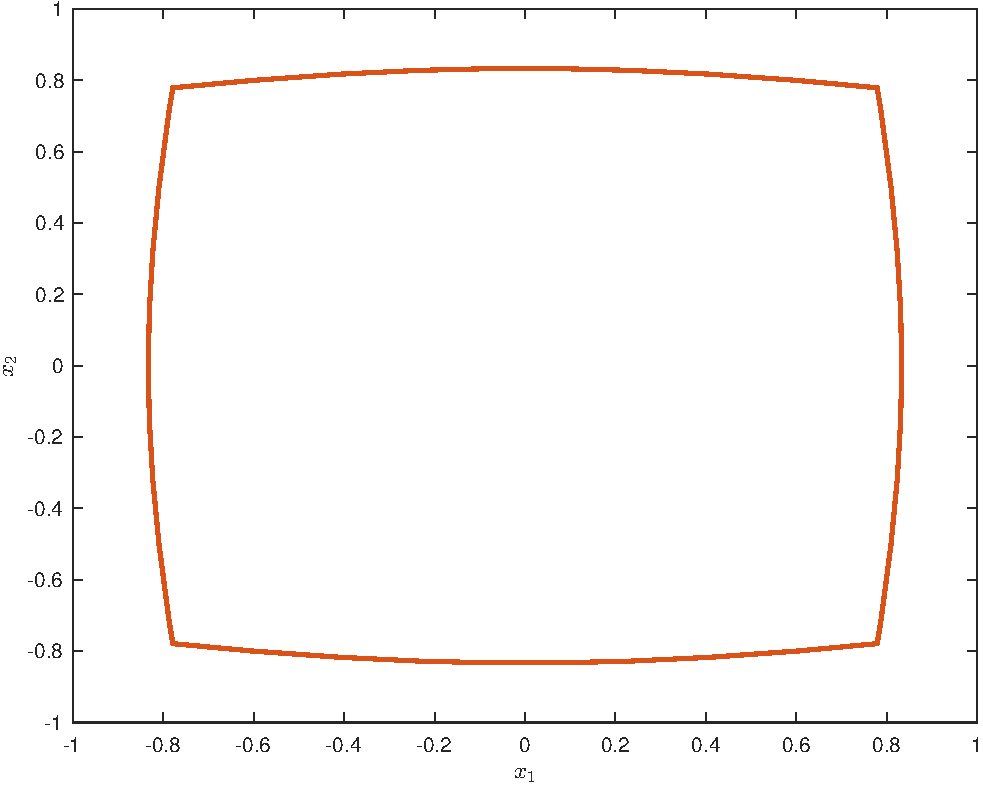
\includegraphics[width=.95\textwidth]{parametricPD.pdf}
\caption{$X\ominus\mathcal W(X)$}
\label{fig:example:parametric:pontryagin:difference}
\end{figure}


\subsection{Element wise bound sets}\label{exp:second:example}
%
For another example we take inspiration from a robust control scenario.
%
We want to approximate the maximal positive invariant set for a system of the type~$x^+=Ax + f(x)$ for $x\in\mathcal X$, i.e. the largest set of points~$\mathcal X^\infty\subseteq\mathcal X$ such that $x\in\mathcal X^\infty\Rightarrow x^+\in\mathcal X^\infty$, see e.g.~\cite{blanchini:2007}.
%
For general nonlinear systems~$x^+=Ax + f(x)$ the maximal positive invariant set can not be calculated, but assume we find piecewise affine bounds on the nonlinearity, i.e. $\min_{k\leq M_i}\{h_{i,k}^x x + h_{i,k}^c\}\leq f_i(x)\leq\max_{k\leq N_i}\{H_{i,k}^x x + H_{i,k}^c\}$ for all $x\in\mathcal X$ and all elements of~$f(x)$.
%
We can now study the system $x^+=Ax+w$ with $w\in\mathcal W(x) = \{w:\min_{k\leq M_i}\{h_{i,k}^x x + h_{i,k}^c\}\leq w_i\leq\max_{k\leq N_i}\{H_{i,k}^x x + H_{i,k}^c\}\,\forall i\in\{1,\dots,d\}\}$.
%
Instead of computing the maximal positive invariant set for the nonlinear system we compute the maximal robust positive invariant set for the perturbed linear system $x^+=Ax+w$, i.e. the set of states~$\mathscr X^\infty\subseteq\mathcal X$ such that $x\in\mathscr X^\infty$ implies $x^+\in\mathscr X^\infty$ for all possible $w\in\mathcal W(x)$.
%
The algorithm to determine the maximal robust positive invariant sets recursively intersects the current set iterate~$X_l$ with the set of all possible successor states starting from the current iterate $X_{l+1}=X_l\cap\left\{\bigcup_{x\in X_l,w\in\mathcal W(x)}\{Ax+w\}\right\}$, we will only present a single step.
%
Notice that for a constant set-valued map~$\mathcal W(x) = \mathcal W$ the iteration can be summarised as $X_{l+1} = X_l\cap A^{-1}(X_l\ominus\mathcal W)$, for a set valued map a similar compact notation also holds, however it is more confusing than helpful:~$X_{l+1}=X_l\cap(A^{-1}X_l\ominus A^{-1}\mathcal W(A^{-1}X_l))$.

In order to illustrate the proposed treatment of the nonlinearities we use the two dimensional system~$x^+=x+f(x)$ where the nonlinearity is given by
%
\begin{subequations}
\begin{equation}
  f_1(x) = \frac{1}{10}\left(\frac{x_1}{2}+x_2\right)^3
\end{equation}
\begin{equation}
  f_2(x) = \frac{1}{2}\arcsin\left(\sigma\left(x_1-\frac{x_2}{2}\right)\sqrt{\frac{x_1-\frac{x_2}{2}}{2}} + \sigma\left(-\left(x_1-\frac{x_2}{2}\right)\right)\frac{x_1-\frac{x_2}{2}}{2} \right)
\end{equation}
\end{subequations}
%
with the Heaviside function
%
$$
  \sigma(t) = \left\{\begin{array}{crcl}1& t&\geq&0\\ 0 &t&<&0 \end{array}\right.
$$
%
As the constraint set we use $X_l = \{x:\abs{x_1}+\abs{x_2}\leq 2\}$.
%
In order not to bore the reader with numerical values, we illustrate the approximation of $f_1(x)$ in Figure~\ref{fig:approximation:f1:p:diff} and~$f_2(x)$ in Figure~\ref{fig:approximation:f2:p:diff}, for both we obtain upper and lower bounds using secants and tangents.
%
Figure~\ref{fig:approximation:f2:p:diff} shows an obvious weakness of the approach:~$\max_k\{c_k x+b_k\}$ is always convex, therefore approximating non-convex functions introduces conservativeness.

The actual computation of the set~$X_{l+1}$ is then done analogous to the previous example, again we use that 
%
$$
  \mathcal W(x) = \conv\left\{\begin{pmatrix}t_1\\ t_3\end{pmatrix},\begin{pmatrix}t_1\\ t_4\end{pmatrix},
  \begin{pmatrix} t_2\\ t_3\end{pmatrix},\begin{pmatrix}t_2\\ t_4\end{pmatrix}
  \right\}
$$
%
with $t_1=\max_k\{H_{1,k}^x x+H_{1,k}^c\},\; t_3=\max_k\{H_{2,k}^x x+H_{2,k}^c\},\; t_2=-\max_k\{-h_{1,k}^x x-h_{1,k}^c\}$ and $t_4=-\max_k\{-h_{1,k}^x x-h_{1,k}^c\}$.
%
Each facet~$P_i=\{x:\Lambda_i x=\lambda_i\wedge\Lambda_jx\leq\lambda_j,j\neq i\}$ of the current set iterate defines facets of the next set iterate satisfying
%
\begin{equation}
\Lambda_i(Ax+w^\ast)=\lambda_i\quad \Lambda_j(Ax+w^\ast)\leq\lambda_j,j\neq i
\end{equation}
%
where $w^\ast$ is the maximiser of the defining mpLP $\max_{w\in\mathcal W(x)}\Lambda_iw$, i.e. one of the aforementioned vertices with their representation
%
$$
  \begin{pmatrix} w_1\\ \vdots \\ w_N\end{pmatrix}= Tt.
$$
%
With this the collection of facets generated by~$P_i$ is given by the projection
%
\begin{equation}
  \pi_d\left(\left\{(x,t,\tau)\in\mathbb R^{3d+1}:\begin{array}{rcl}
  \Lambda_iAx+\tau&=&\lambda_i\\
  \Lambda_i T_lt&\leq&\tau\\
  \Lambda_j(Ax+T_lt)&\leq&\lambda_j\\
  H_l^x x + H_l^c&\leq&t_{2l-1}\\
  -h_l^x x - h_l^c&\leq&t_{2l}
  \end{array}, \begin{array}{l}
  j\neq i\\
  l\in\{1,\dots,d\}\end{array}
  \right\}\right)
\end{equation}
%
Analogous to the previous example, instead of computing~$q$ projections from $3d+1$ onto $d$ we can perform a single projection with the same result:
%
\begin{equation}
  \pi_d\left(\left\{(x,t,\tau)\in\mathbb R^{3d+q}:\begin{array}{rcl}
  \Lambda_i T_lt&\leq&\tau_i\\
  \Lambda_iAx+\tau_i&\leq&\lambda_i\\
  H_l^x x + H_l^c&\leq&t_{2l-1}\\
  -h_l^x x - h_l^c&\leq&t_{2l}
  \end{array}, \begin{array}{l}
  i\in\{1,\dots,q\},\\
  l\in\{1,\dots,d\}\end{array}
  \right\}\right)
\end{equation}
%
The resulting set for our 2 dimensional example is illustrated in Figure~\ref{fig:second:example:resulting:set}.


\begin{figure}
\centering
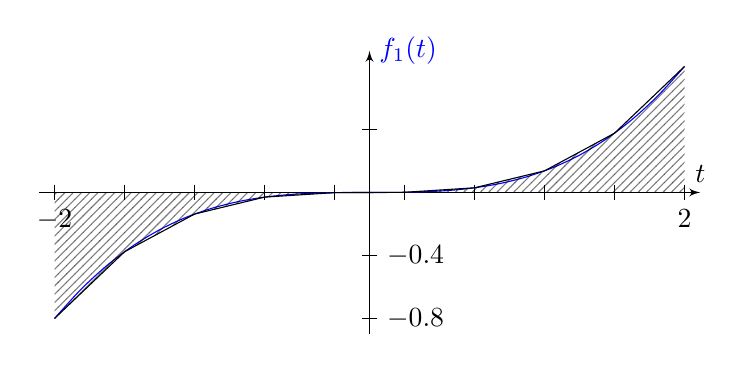
\begin{tikzpicture}[scale=2]
\draw[-latex'] (-2.1,0) -- (2.1,0) node[above] {$t$};
\draw[-latex'] (0,-.9) -- (0,.9) node[right,blue] {$f_1(t)$};
\foreach \x in {-2,-1.5556,...,2} \draw (\x,0.05) -- (\x,-.05);
\draw (-2,-.05) node[below] {$-2$};
\draw (2,-.05) node[below] {$2$};
\foreach \y in {-.8,-.4,...,.8} \draw (0.05,\y) -- (-.05,\y);
\draw (.05,-.8) node[right] {$-0.8$};
\draw (.05,-.4) node[right] {$-0.4$};
\draw[scale=1,domain=-2:2,smooth,variable=\x,blue] plot ({\x},{\x*\x*\x/10});
\draw (-2.0000, -0.8000) -- (-1.5556, -0.3764) -- (-1.1111, -0.1372) -- (-0.6667, -0.0296) -- (-0.2222, -0.0011) -- (0,0); 
\draw (0,0) -- (0.2222, 0.0011) -- (0.6667, 0.0296) -- (1.1111, 0.1372) -- (1.5556, 0.3764) -- (2.0000, 0.8000);
\fill[pattern = north east lines, opacity=.5] (-2.0000, -0.8000) -- (-1.5556, -0.3764) -- (-1.1111, -0.1372) -- (-0.6667, -0.0296) -- (-0.2222, -0.0011) -- (0,0) -- (-2,0) -- cycle; 
\fill[pattern = north east lines, opacity=.5] (0,0) -- (0.2222, 0.0011) -- (0.6667, 0.0296) -- (1.1111, 0.1372) -- (1.5556, 0.3764) -- (2.0000, 0.8000) -- (2,0) -- cycle;
\end{tikzpicture}
\caption{$f_1(t=\frac{x_1}{2}+x_2)$ and its approximation by 9 secants used in Example~\ref{exp:second:example}.}
\label{fig:approximation:f1:p:diff}
\end{figure}

\begin{figure}
\centering
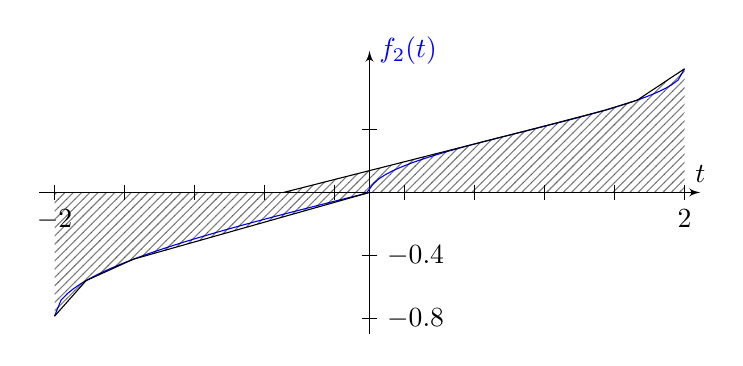
\begin{tikzpicture}[scale=2]
\draw[-latex'] (-2.1,0) -- (2.1,0) node[above] {$t$};
\draw[-latex'] (0,-.9) -- (0,.9) node[right,blue] {$f_2(t)$};
\foreach \x in {-2,-1.5556,...,2} \draw (\x,0.05) -- (\x,-.05);
\draw (-2,-.05) node[below] {$-2$};
\draw (2,-.05) node[below] {$2$};
\foreach \y in {-.8,-.4,...,.8} \draw (0.05,\y) -- (-.05,\y);
\draw (.05,-.8) node[right] {$-0.8$};
\draw (.05,-.4) node[right] {$-0.4$};
\draw[blue] (-2.0000, -0.7854) -- (-1.9596, -0.6847) -- (-1.9192, -0.6428) -- (-1.8788, -0.6104) -- (-1.8384, -0.5830) -- (-1.7980, -0.5587) -- (-1.7576, -0.5367) -- (-1.7172, -0.5163) -- (-1.6768, -0.4972) -- (-1.6364, -0.4791) -- (-1.5960, -0.4620) -- (-1.5556, -0.4456) -- (-1.5152, -0.4298) -- (-1.4747, -0.4146) -- (-1.4343, -0.3999) -- (-1.3939, -0.3856) -- (-1.3535, -0.3717) -- (-1.3131, -0.3581) -- (-1.2727, -0.3449) -- (-1.2323, -0.3319) -- (-1.1919, -0.3192) -- (-1.1515, -0.3068) -- (-1.1111, -0.2945) -- (-1.0707, -0.2825) -- (-1.0303, -0.2706) -- (-0.9899, -0.2589) -- (-0.9495, -0.2473) -- (-0.9091, -0.2359) -- (-0.8687, -0.2247) -- (-0.8283, -0.2135) -- (-0.7879, -0.2025) -- (-0.7475, -0.1915) -- (-0.7071, -0.1807) -- (-0.6667, -0.1699) -- (-0.6263, -0.1592) -- (-0.5859, -0.1486) -- (-0.5455, -0.1381) -- (-0.5051, -0.1276) -- (-0.4646, -0.1172) -- (-0.4242, -0.1069) -- (-0.3838, -0.0966) -- (-0.3434, -0.0863) -- (-0.3030, -0.0761) -- (-0.2626, -0.0658) -- (-0.2222, -0.0557) -- (-0.1818, -0.0455) -- (-0.1414, -0.0354) -- (-0.1010, -0.0253) -- (-0.0606, -0.0152) -- (-0.0202, -0.0051) -- ( 0.0202,  0.0503) -- ( 0.0606,  0.0875) -- ( 0.1010,  0.1133) -- ( 0.1414,  0.1346) -- ( 0.1818,  0.1531) -- ( 0.2222,  0.1699) -- ( 0.2626,  0.1854) -- ( 0.3030,  0.1999) -- ( 0.3434,  0.2136) -- ( 0.3838,  0.2267) -- ( 0.4242,  0.2393) -- ( 0.4646,  0.2515) -- ( 0.5051,  0.2633) -- ( 0.5455,  0.2747) -- ( 0.5859,  0.2859) -- ( 0.6263,  0.2969) -- ( 0.6667,  0.3077) -- ( 0.7071,  0.3184) -- ( 0.7475,  0.3289) -- ( 0.7879,  0.3393) -- ( 0.8283,  0.3496) -- ( 0.8687,  0.3598) -- ( 0.9091,  0.3699) -- ( 0.9495,  0.3801) -- ( 0.9899,  0.3902) -- ( 1.0303,  0.4003) -- ( 1.0707,  0.4104) -- ( 1.1111,  0.4205) -- ( 1.1515,  0.4307) -- ( 1.1919,  0.4410) -- ( 1.2323,  0.4513) -- ( 1.2727,  0.4618) -- ( 1.3131,  0.4723) -- ( 1.3535,  0.4830) -- ( 1.3939,  0.4939) -- ( 1.4343,  0.5050) -- ( 1.4747,  0.5164) -- ( 1.5152,  0.5280) -- ( 1.5556,  0.5400) -- ( 1.5960,  0.5523) -- ( 1.6364,  0.5651) -- ( 1.6768,  0.5785) -- ( 1.7172,  0.5926) -- ( 1.7576,  0.6076) -- ( 1.7980,  0.6237) -- ( 1.8384,  0.6413) -- ( 1.8788,  0.6610) -- ( 1.9192,  0.6842) -- ( 1.9596,  0.7141) -- ( 2.0000,  0.7854);
\draw (-2.0000, -0.7854) -- (-1.8000, -0.5599) -- (-1.5000, -0.4240) -- (0, 0);
\fill[pattern = north east lines, opacity=.5] (-2.0000, -0.7854) -- (-1.8000, -0.5599) -- (-1.5000, -0.4240) -- (0, 0) -- (-2,0) -- cycle;
\draw (-.5466,0) -- (0.7000, 0.3165) -- (1.0000, 0.3927) -- (1.5000, 0.5236) -- (1.7000, 0.5865) -- (2.0000, 0.7854);
\fill[pattern = north east lines, opacity=.5] (-.5466,0) -- (0.7000, 0.3165) -- (1.0000, 0.3927) -- (1.5000, 0.5236) -- (1.7000, 0.5865) -- (2.0000, 0.7854) -- (2,0) -- cycle;
\end{tikzpicture}
\caption{$f_2(t=x_1-\frac{x_2}{2})$ and its approximation by 5 secants and 4 tangents as used in Example~\ref{exp:second:example}.}
\label{fig:approximation:f2:p:diff}
\end{figure}

\begin{figure}
\centering
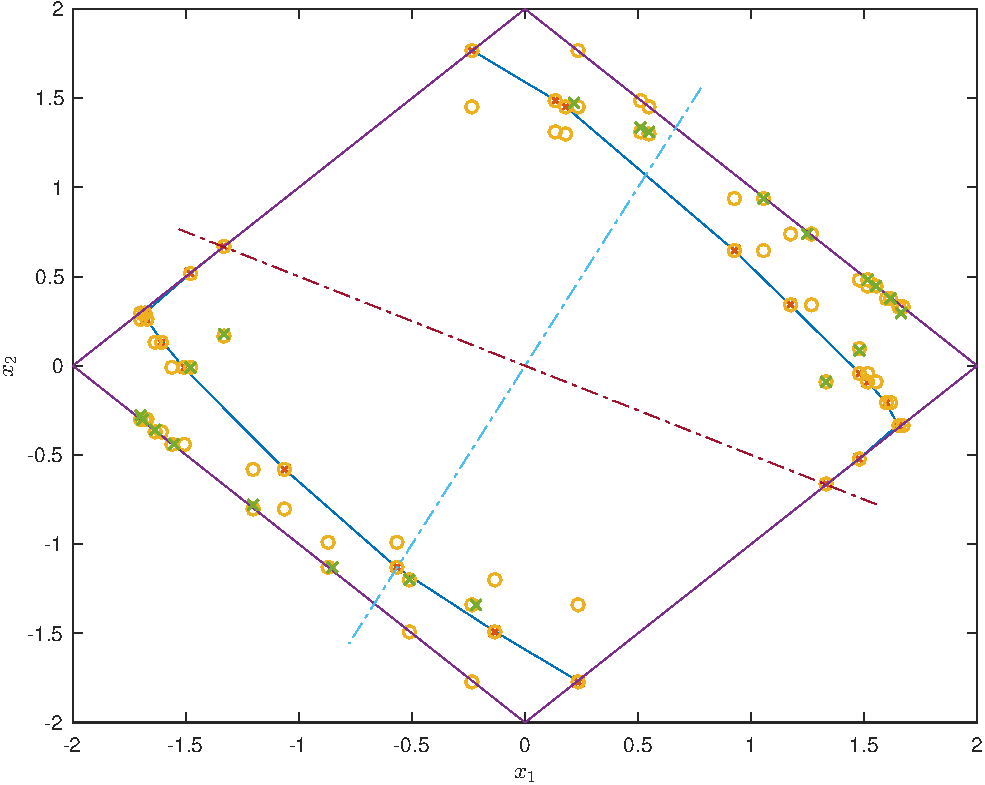
\includegraphics[width=.95\textwidth]{complexPonDiff.pdf}
\caption{In purple~$X_l$, outlined in blue~$X_{l+1}$, its vertices~$v_i$ marked by red crosses, yellow circles mark the vertices of $\{v_i\}\oplus\mathcal W(v_i)$, green crosses mark the actual value of $f(v_i)$ and dotted lines show the $x_1-\frac{x_2}{2}=0$ and $\frac{x_1}{2}+x_2=0$ planes.}
\label{fig:second:example:resulting:set}
\end{figure}


\section*{References}

\bibliography{Bibliography}

\end{document}